\chapter{Estrutura do Projeto}
\label{sec:estrutura}

\setcounter{defcnt}{0}

  No capítulo anterior revisamos e apresentamos conceitos visando responder a
  pergunta ``Como integrar \CXX{} com linguagens de \script{}?''. Agora que
  temos essas ferramentas a nosso dispor, vamos modelar uma solução. Para isso
  precisamos entender, em termos práticos, o que nosso sistema deve ser capaz
  de fazer, e então projetar uma estrutura que satisfaça esses requisitos.
  
  Um usuário do nosso sistema estará tipicamente desenvolvendo uma aplicação
  em \CXX{} que de alguma forma precisa ser capaz de interagir com \lang{Lua}
  e \lang{Python}, possivelmente ambas ao mesmo tempo. Como vimos na sessão
  \ref{cap:conceitos:maquina}, essa interação pode ser estabelecida de maneira
  bastante direta entre elas se a máquina virtual da linguagem de \script{} em
  questão tiver sido programada na linguagem compilada em questão. Para evitar
  repetitividade e simplificar o texto, diremos, do ponto de vista das
  máquinas virtuais envolvidas, que:

  \definicao{
    \vspace{-1.5em}
    \begin{enumerate}
      \item A \textbf{linguagem nativa} é a linguagem na qual a máquina
            virtual foi implementada.
      \item A \textbf{linguagem virtual} é a linguagem que a máquina virtual
            processa para executar suas simulações.
    \end{enumerate}
  }

  Ou seja, \CXX{} será a nossa linguagem nativa de interesse, enquanto que
  as linguagens virtuais serão \lang{Lua} e \lang{Python}, mas também poderiam
  ser quaisquer outras linguagens cujas máquinas virtuais estejam programadas em
  \C{} ou \CXX{}.

  \section{Visão Geral}
  \label{sec:estrutura:geral}

    Para auxiliar a modelagem da estrutura, vamos dizer que tanto a aplicação
    quantos os \script{s} estão divididos em \textbf{módulos}. Eles serão os
    objetos que representam o conjunto de elementos provenientes de uma ou de
    outra linguagem que podem ser acessados e manipulados. Por exemplo, se a
    aplicação em questão for um jogo de ação no qual o jogador enfrenta inimigos
    virtuais, o desenvolvedor poderia usar \script{s} para implementar a
    inteligência artifical desse inimigos, para que fosse fácil ajustá-las sem
    ter que recompilar o jogo. Desse modo, cada um desses \script{s} seria um
    módulo que a aplicação precisaria carregar e usar durante sua execução.
    Eles, por sua vez, precisariam interagir com módulos da aplicação para que
    as inteligências artificiais conseguissem manipular seus personagens dentro
    do mundo virtual do jogo. Se elas quisessem saber o quão próximo o herói
    está, elas precisariam usar as funções do módulo de controle de
    posicionamento dos avatares. Se elas quisessem criar um projétil para atacar
    o jogador, elas precisariam acessar o módulo que contenha a
    classe\footnotemark{} que representa o projétil desejado.

    \footnotetext{
      Classes são estruturas presentes em linguagens de programação
      \emph{orientadas a objetos}. Seu papel é definir os dados e os
      comportamentos que um conjunto de objetos deve ter.
    }

    \begin{figure}[ht]
      \centering
      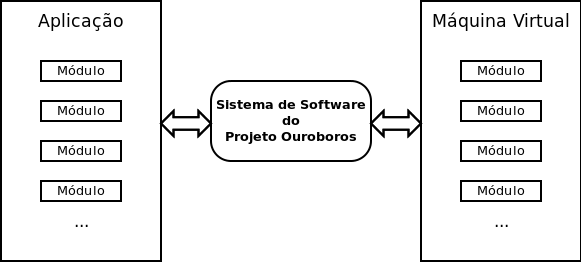
\includegraphics[width=.8\textwidth]{overview-simple.png}
      \caption{Esquematização bem simplificada do funcionamento sistema.}
      \label{fig:overview-simple}
    \end{figure}

    Dessa forma, uma primeira ilustração bem simplificada do funcionamento do
    nosso sistema é a representada na Figura \ref{fig:overview-simple}. O
    sistema Ouroboros será responsável por fornecer acesso aos módulos entre a
    aplicação e as máquinas virtuais. Dessa forma, estabelecemos duas
    grandes funcionalidades no sistema: providenciar à aplicação a possibilidade
    de manipular os módulos das máquinas virtuais, e deixar os módulos da
    aplicação à disposição dos \script{s} . Esses processos são conhecidos como
    \textbf{incorporação}\footnote{Do inglês, ``\textit{embedding}''.} e
    \textbf{exportação}, respectivamente.

    \definicao{
      \vspace{-1.5em}
      \begin{enumerate}
        \item \textbf{Incorporação} é quando a aplicação programada na linguagem
              nativa pode acessar e manipular os elementos dos módulos da
              máquina virtual.
        \item \textbf{Exportação} é quando módulos da aplicação na linguagem
              nativa são registrados na máquina virtual de modo que os módulos
              desta possam usar funcionalidades daquela.
      \end{enumerate}
    }

    Nesse ponto vale à pena destacar um aspecto que ficou de lado até agora.
    Como o subtítulo desse trabalho indica, o propósito do sistema é não só
    integrar as ditas linguagens, como fazê-lo de maneira \textit{automatizada}.
    Até porque as APIs das máquinas virtuais por sí sós possuem seus próprios
    mecanismos de fornecer incorporação e exportação, indicando que nosso
    projeto seria redundante, não fosse o fato que elas são trabalhosas e
    específicas demais de usar. A intenção é que o usuário do nosso sistema não
    tenha que se preocupar com os detalhes de cada máquina virtual quando
    estiver desenvolvendo a aplicação dele e seja capaz de escrever normalmente
    os \script{s} que trabalhem com ela - isso é, podendo acessar módulos
    externos através dos mecanismos usuais que a linguagem virtual fornece.

    Logo, nosso sistema consistirá majoritariamente de uma biblioteca \CXX{}
    que disponibiliza incorporação e exportação automatiza de e para \script{s}.
    Faremos isso aproveitando as possibilidades de abstração da linguagem
    escolhida para encapsular os comportamentos desejados. As duas próximas
    sessões explicarão como projetamos as partes dessa biblioteca que atenderão
    cada um desses requisitos.

  \section{API unificada para incorporação de \script{s}}
  \label{sec:estrutura:opa}

    Como vimos na sessão \ref{cap:conceitos:apis}, as máquinas virtuais com que
    estamos trabalhando possuem um API própria através da qual podemos manipular
    seu conteúdo. Para evitar que o usuário acesse elas diretamente, podemos
    ocultá-las por trás de uma camada que constitua uma nova API. Ela unificará
    o acesso às funcionalidades de todas as máquinas virtuais compatíveis. Mais
    especificamente, ela fornecerá os seguintes serviços:

    % TODO: Diagrama ilustrando relação da OPA com as APIs específicas de cada
    %       linguagem de script

    \begin{itemize}
      \item Carregar um módulo a partir de um \script{};
      \item Executar rotinas implementadas na linguagem virtual;
      \item Obter e/ou alterar valores de variáveis, objetos e atributos
            definidos na linguagem virtual;
      \item Converter valores entre tipos da linguagem nativa e tipos da
            linguagem virtual;
    \end{itemize}

    Idealmente, quando o usuário requisitar um desses serviços, ele não precisa
    saber qual máquina virtual realmente vai atendê-lo. Em termos práticos, isso
    significa que quando ele evocar a rotina desejada, queremos que na verdade a
    rotina executada seja aquela que corresponda à máquina virtual apropriada
    ``sem que ele perceba''. Ou seja, precisamos de funções com nomes e
    assinaturas\footnotemark{} fixos representando a operação almejada, porém
    sobrecarregadas com implementações circunstancialmente diferentes. Um jeito
    de obter esse efeito em \CXX{} é através da herança de classes, que é o
    método que adotamos.

    \footnotetext{
      A \emph{assinatura} de uma rotina ou função especifica que tipos de
      parâmetros ela recebe e que tipos de valores ela devolve a quem a
      evocou.
    }

    %TODO: usar o parágrafo abaixo para explicar as principais classes que o
    %      sistema precisa ter para suportar incorporação

    Uma parte dessa API é uma interface polimórfica que, ao ser implementada usando
    as rotinas da máquina virtual de uma linguagem de \script{}, possibilita que
    a \emph{libouroboros} reconheça e trabalhe com tal linguagem. Essa
    implementação deve satisfazer nossa interface, isso é, as operações
    descritas acima. A nossa API administrará as diversas implementações
    disponíveis apresentando ao usuário final da OPA apenas a interface
    unificada. Desse jeito, ele não precisa saber sobre esse gerenciamento
    interno, nem se preocupar com a API da linguagem de \script{}, a não ser que
    seja ele quem vá adicionar o suporte a ela no sistema.
    
    %TODO: subsection: conversão de valores (entre linguagem nativa e máquina virtual)
    %TODO: subsection: virtualobj (possiveis subsubsection pra falar do encapsulamento do vdata, etc)
    %TODO: subsection: importação de um módulo de script para a linguagem nativa
  
  
  \section{Gerador de \emph{wrappers} e interfaces.}
  \label{sec:estrutura:opwig}

  %TODO: Explicar mais sobre a ideia geral da relação do tipo (B)

    Linguagens de \script{} possuem um mecanismo próprio para incluir módulos
    externos, eventualmente necessários à sua execução. Esses módulos podem ser
    definidos tanto em outros arquivos na mesma linguagem, quanto na linguagem
    nativa da máquina virtual. Nesse último caso, temos a relação do tipo (B). Ela
    exige que a linguagem nativa disponibilize certos dados seguindo um protocolo
    adequado. Infelizmente tal protocolo não só difere para cada linguagem de
    \script{} como também involve um trabalho repetitivo e maçante para ser utilizado. 

    %TODO: Detalhar esse processo repetitivo e maçante.
    
    Por isso, parte do nosso sistema é composto por um gerador automatizado de código fonte.
    Ele é responsável por criar o código necessário à devida exportação dos módulos 
    feitos na linguagem nativa. Além disso, ele processa código que o usuário fornecer na
    linguagem nativa para saber o conteúdo que deve aparecer no módulo exportado.
    Esse conteúdo é inserido no módulo através de \emph{wrappers}. Chamamos esse componente
    do sistema de \emph{Ouroboros Project Wrapper and Interface Generator} (OPWIG).
  
    %TODO: subsection: parser
    %TODO: subsection: code generator
    %TODO: subsection: wrapper explanation 
  
  \section{Integrando e entregando tudo para o usuário.}
  \label{sec:estrutura:integration}

    Isso será escrito na versão final da monografia.
